\scanpage{14}
\mspage{3}

\figure{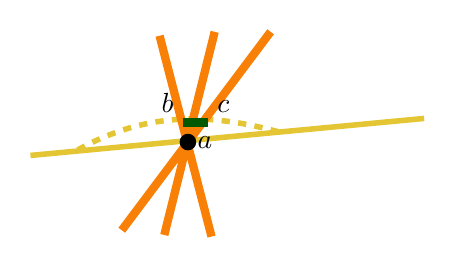
\begin{tikzpicture}[x=1cm,y=1cm]
\draw[yellow!55!brown,line width=2pt] (-2,-.17)--(3,.30);
\draw[yellow!55!brown,line width=2pt,dashed] (-1.4,-.1) .. controls(-.5,.40) and (.3,.36).. (1.15,.13);
\draw[orange!90!brown,line width=3pt] (-.36,1.35)--(.30,-1.2) (.34,1.40)--(-.30,-1.18) (1.05,1.40)--(-.84,-1.12);
\draw[black!65!green,line width=3pt] (-.06,.25)--(.25,.25);
\fill (0,0) circle(3pt);\node[right] at (0,0){$a$};\node[above left] at (-.06,.25){$b$};\node[above right] at (.25,.25){$c$};
\end{tikzpicture}}

spécialisation $(abc)$ de $D'$. Il y a au moins deux autres triangles de spécialisation pour $D'$, qui auront une base sur $D'$ \deleted{qui} qui rencontre $(b,c)$ au plus en un sommet. Si l'un d'eux ne contient ni $b$ ni $c$, on a gagné. Sinon, on a la figure

\margin{\deleted{\unsure{mais?}} \deleted{\unsure{fausse!}}}

\figure{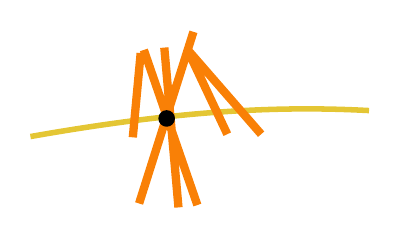
\begin{tikzpicture}[x=1cm,y=1cm]
\draw[yellow!55!brown,line width=2pt] (-1.7,-.15) .. controls(0,.15) and (1.3,.25)..(2.6,.18);
\draw[orange!90!brown,line width=3pt] (-.26,.95)--(.42,-1.02) (0,.98)--(.18,-1.05) (.37,1.18)--(-.32,-1.00) (-.30,.91)--(-.40,-.16) (.29,.96)--(.80,-.12) (.29,.96)--(1.23,-.12);
\fill (.03,.08) circle(3pt);
\end{tikzpicture}}

\figure{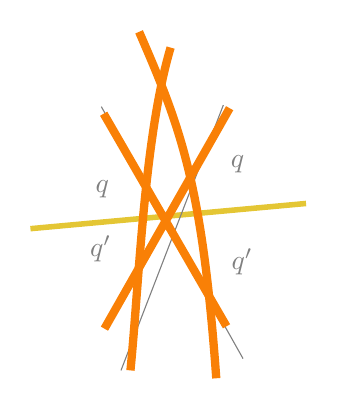
\begin{tikzpicture}[x=1cm,y=1cm]
\draw[yellow!55!brown,line width=2pt] (-1.8,-.10)--(1.7,.22);
\draw[gray,thin] (-.9,1.45)--(.9,-1.75) (.65,1.47)--(-.65,-1.9);
\draw[orange!90!brown,line width=3pt] (-.42,2.40) .. controls(.10,1.20) and (.38,.50)..(.56,-2.0);
\draw[orange!90!brown,line width=3pt] (-.02,2.20) .. controls(-.36,1.05) and (-.42,-.8)..(-.53,-1.9);
\draw[orange!90!brown,line width=3pt] (-.87,1.36)--(.69,-1.34) (.73,1.43)--(-.86,-1.37);
\node[gray,left] at (-.68,.40){$\unsure{q}$};\node[gray,right] at (.62,.72){$\unsure{q}$};\node[gray,left] at (-.65,-.35){$\unsure{q'}$};\node[gray,right] at (.63,-.52){$\unsure{q'}$};
\end{tikzpicture}}

Il y a effectivement un contre-exemple avec $\Sigma=\unsure{\mathrm{St}_4}$, et $D$ \deleted{\unsure{dans}} la position sous-stable qui évite les deux couloirs incidents à $a$, et coupe longitudinalement le troisième.

Mais je m'aperçois que dans la description de l'ens des sommets $P=\operatorname{PR}(\Sigma)$ de $\Gamma$, j'ai oublié les cas les plus importants --- les p.r. \uline{supercritiques}, correspondant aux droites de $\Sigma$ lui-$=$! Il faut que je décrive alors quelles sont les spécialisations vers un tel $\Delta$. Il est clair qu'elles \unsure{ne doit|ne dvt} se faire à \uline{partir d'une position stable} \inserted{(car ce sont des spécialisations \uline{immédiates},)} au contraire --- on doit avoir $\operatorname{Card}(S\cap D)=1$ i.e. $D$ sous-stable. Soit $S\cap D=\{a\}$, il faut que $a$ soit un sommet de $\Delta$, d'autre part, il doit y avoir un secteur biangulaire global dans $X$, défini par $D,\Delta$, qui soit un ``\uline{couloir}'' et la spécialisation se fait en suivant ce couloir, qu'on pourrait nommer \uline{couloir de spécialisation}.

\figure{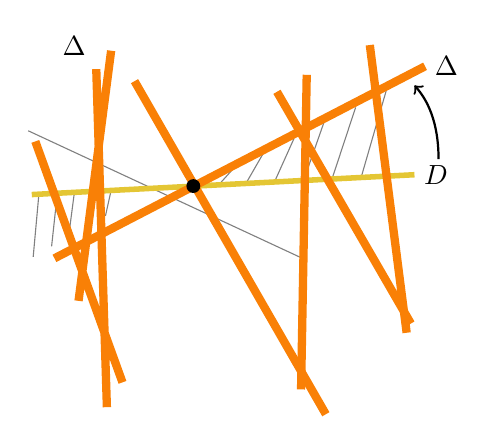
\begin{tikzpicture}[x=.9cm,y=.9cm]
\draw[gray,thin] (-2.45,.80)--(1.42,-1.0);
\draw[gray,thin] (-2.3,-.1)--(-2.38,-.98) (-2.04,-.09)--(-2.12,-.83) (-1.80,-.08)--(-1.88,-.69) (-1.55,-.06)--(-1.63,-.53) (-1.28,-.04)--(-1.36,-.40);
\draw[gray,thin] (.25,.05)--(.43,.25) (.63,.07)--(.86,.47) (1.03,.09)--(1.30,.69) (1.44,.11)--(1.72,.91) (1.84,.13)--(2.17,1.13) (2.25,.15)--(2.60,1.36);
\draw[yellow!55!brown,line width=2pt] (-2.4,-.1)--(3.0,.18);
\draw[orange!90!brown,line width=3pt] (-2.08,-1.00)--(3.15,1.71);
\draw[orange!90!brown,line width=3pt] (-2.35,.65)--(-1.12,-2.75) (-1.28,1.93)--(-1.74,-1.60) (-1.49,1.67)--(-1.34,-3.10) (-.95,1.50)--(1.75,-3.2);
\draw[orange!90!brown,line width=3pt] (1.06,1.35)--(2.95,-1.92) (1.48,1.59)--(1.40,-2.85) (2.37,2.01)--(2.89,-2.05);
\fill (-.12,.02) circle(2.5pt);
\node[above left] at (-1.5,1.72){$\Delta$};\node[right] at (3.15,1.71){$\Delta$};\node[right] at (3,.18){$D$};
\draw[->,thick] (3.34,.40) .. controls(3.34,.93) and (3.18,1.24)..(3.00,1.44);
\end{tikzpicture}}

Il peut y avoir aussi un couloir de spécialisation, sur chaque \unsure{vis} de $D\setminus\{a\}$. Quoi qu'il en soit, on considérera les couloirs de spécialisation \inserted{pour $D$} comme ``équivalents'' à un triangle de sp. pour $D$.

\margin{13}
